\documentclass[11pt]{article}

%------------------------- fonts & encoding -----------------------------------
\usepackage[T1]{fontenc}
\usepackage[utf8]{inputenc}
\usepackage{amsmath,amssymb,amsthm}
\usepackage{mathtools}
\usepackage[sc]{mathpazo}
\linespread{1.06}
\usepackage{microtype}

%------------------------- layout ---------------------------------------------
\usepackage[a4paper,margin=1.05in,marginparwidth=1.0in]{geometry}
\usepackage{booktabs}
\usepackage{enumitem}
\setlist{itemsep=2pt,topsep=3pt}
\usepackage{xcolor}
\usepackage{graphicx}
\usepackage{tikz}
\usepackage{pgfplots}
\pgfplotsset{compat=1.17}
\usepackage[most,breakable]{tcolorbox}

%------------------------- palette --------------------------------------------
\definecolor{crimson}{HTML}{A51C30}
\definecolor{ink}{HTML}{1A1A1A}
\definecolor{steel}{HTML}{2C5F8A}
\definecolor{amber}{HTML}{9A6A00}
\definecolor{teal}{HTML}{1F6F6B}
\definecolor{paperlt}{HTML}{F7F4EF}

%------------------------- section styling ------------------------------------
\usepackage{titlesec}
\titleformat{\section}{\Large\bfseries\color{steel}}{\thesection}{0.7em}{}
\titleformat{\subsection}{\large\bfseries\color{ink}}{\thesubsection}{0.6em}{}
\titlespacing*{\section}{0pt}{1.6em}{0.6em}

%------------------------- hyperref -------------------------------------------
\usepackage[colorlinks=true,linkcolor=steel,citecolor=steel,urlcolor=crimson]{hyperref}

%------------------------- theorem environments -------------------------------
\theoremstyle{definition}
\newtheorem{definition}{Definition}[section]
\newtheorem{example}{Example}[section]
\newtheorem{exercise}{Exercise}[section]
\theoremstyle{plain}
\newtheorem{proposition}{Proposition}[section]
\theoremstyle{remark}
\newtheorem*{remark}{Remark}

%------------------------- callout boxes --------------------------------------
\newtcolorbox{intuition}{
  enhanced, breakable, colback=crimson!5, colframe=crimson, boxrule=0.4pt,
  left=8pt,right=8pt,top=6pt,bottom=6pt, arc=2pt,
  borderline west={2.5pt}{0pt}{crimson},
  fonttitle=\bfseries\color{crimson}, title={Intuition}}

\newtcolorbox{pitfall}{
  enhanced, breakable, colback=amber!7, colframe=amber, boxrule=0.4pt,
  left=8pt,right=8pt,top=6pt,bottom=6pt, arc=2pt,
  borderline west={2.5pt}{0pt}{amber},
  fonttitle=\bfseries\color{amber}, title={What goes wrong}}

\newtcolorbox{keyresult}{
  enhanced, breakable, colback=steel!6, colframe=steel, boxrule=0.5pt,
  left=8pt,right=8pt,top=6pt,bottom=6pt, arc=2pt,
  fonttitle=\bfseries\color{steel}, title={Takeaway}}

\newtcolorbox{observed}{
  enhanced, breakable, colback=teal!6, colframe=teal, boxrule=0.4pt,
  left=8pt,right=8pt,top=6pt,bottom=6pt, arc=2pt,
  borderline west={2.5pt}{0pt}{teal},
  fonttitle=\bfseries\color{teal}, title={What the pipeline measured}}

%------------------------- math operators -------------------------------------
\DeclareMathOperator{\Var}{Var}
\DeclareMathOperator{\Cov}{Cov}
\DeclareMathOperator{\Corr}{corr}
\DeclareMathOperator{\diag}{diag}
\DeclareMathOperator{\std}{std}
\DeclareMathOperator*{\avg}{\mathbb{E}}
\newcommand{\T}{^{\!\top}}
\newcommand{\R}{\mathbb{R}}
\newcommand{\half}{\tfrac12}
\newcommand{\wvec}{\mathbf{w}}
\newcommand{\Xmat}{\mathbf{X}}
\newcommand{\Fmat}{\mathbf{F}}
\newcommand{\Vmat}{\mathbf{V}}
\newcommand{\Umat}{\mathbf{U}}
\newcommand{\Rmat}{\mathbf{R}}
\newcommand{\Lam}{\boldsymbol{\Lambda}}
\newcommand{\Del}{\boldsymbol{\Delta}}
\newcommand{\fvec}{\mathbf{f}}

%------------------------- title ----------------------------------------------
\title{\vspace{-2.2em}
  {\color{steel}\rule{\textwidth}{1.3pt}}\\[0.7em]
  \Huge\bfseries The Estimation Universe\\[0.35em]
  \large\mdseries The universe every factor is measured against\\[0.4em]
  {\color{steel}\rule{\textwidth}{0.7pt}}}
\author{\textsc{Mathematical Finance}\\[0.2em]
  \small Risk modelling}
\date{}

%------------------------- watermark footer -----------------------------------
\usepackage{fancyhdr}
\pagestyle{fancy}
\fancyhf{}
\renewcommand{\headrulewidth}{0pt}
\renewcommand{\footrulewidth}{0pt}
\fancyfoot[L]{\footnotesize\color{black!45}MSCI Barra USE4 Imitation}
\fancyfoot[R]{\footnotesize\color{black!45}\thepage}

\begin{document}
\maketitle
\thispagestyle{empty}

\begin{abstract}
The \emph{estimation universe} (ESTU) is the set of stocks on which the USE4 model is estimated --- not the (far larger) coverage universe of stocks that ultimately receive exposures and risk forecasts. It is the most quietly load-bearing object in the whole pipeline: a single ESTU sets the standardisation moments for every descriptor, the market benchmark that Beta is measured against, the sample for the cross-sectional regression that backs out factor returns, and the sample for every orthogonalisation regression. Because all four share the same set, an error here does not produce one bug; it biases every factor in a \emph{correlated} way. The awkward fact is that USE4 specifies almost no numerics for the ESTU: it adopts the MSCI USA IMI and defers the actual construction to the proprietary MSCI GIMI methodology. Our organising principle, then, is to reproduce MSCI's three \emph{published} principles --- representation, liquidity, and stability --- as three transparent screens over observable Sharadar data. This set develops those three screens one at a time, shows what the real build measured, and is honest about the one limitation (total- rather than float-adjusted market cap) that we cannot yet close.
\end{abstract}

\begin{tcolorbox}[colback=paperlt,colframe=ink!30,boxrule=0.4pt,arc=2pt,left=10pt,right=10pt,top=8pt,bottom=8pt]
\textbf{How to read these notes.} This is Set~2 of the library, and the first written; read it top to bottom once. The spine is simple: Section~\ref{sec:why} argues why the ESTU matters; Sections~\ref{sec:spec}--\ref{sec:gap} set up what USE4 specifies and the data gap; Sections~\ref{sec:rep}--\ref{sec:stab} build the three screens (representation, liquidity, stability), one concept per section, each independently readable; Sections~\ref{sec:run}--\ref{sec:summary} report the build and close with one honest caveat.

Four coloured boxes recur. \textcolor{crimson}{\textbf{Intuition}} gives the \emph{why} --- mental models and what an object really is. \textcolor{amber}{\textbf{What goes wrong}} shows what breaks \emph{without} the fix, usually by how an optimiser or estimator exploits the modelling error. \textcolor{steel}{\textbf{Takeaway}} flags load-bearing results to retain. \textcolor{teal}{\textbf{What the pipeline measured}} reports \emph{real} numbers from the build run and nothing else.

\textbf{Reference material.}
\begin{itemize}[nosep,leftmargin=1.4em]
  \item \textbf{External:} Menchero, Orr \& Wang (2011), \emph{USE4 Methodology Notes} and \emph{Empirical Notes}, Sec.\ 3.1 and 2.3; the MSCI Global Investable Market Indexes (GIMI) Methodology.
\end{itemize}
\end{tcolorbox}

\tableofcontents
\bigskip

\section{The estimation universe, and why it is load-bearing}\label{sec:why}

\paragraph{Learning objectives.}
\begin{itemize}[nosep,leftmargin=1.4em]
  \item Distinguish the \emph{estimation} universe from the \emph{coverage} universe, and state which stocks contribute to estimating factor returns.
  \item List the four downstream objects the ESTU fixes, and explain why an ESTU error is correlated rather than isolated.
  \item Recall the three published MSCI principles that we will implement as three screens.
\end{itemize}

A risk model has two distinct universes, and conflating them is the most common conceptual error in this whole exercise. The \textbf{coverage universe} $U_t$ is every stock that receives an exposure vector and a risk forecast --- in practice tens of thousands of names. The \textbf{estimation universe} (ESTU) $E_t \subseteq U_t$ is the much smaller set actually \emph{used to estimate the model}: to compute the standardisation moments, to run the cross-sectional regression that backs out factor returns, and to fit the orthogonalisation regressions. A stock outside the ESTU still gets a forecast --- we apply the estimated factor structure to its exposures --- but it does not get a vote in \emph{estimating} that structure.

Why restrict estimation at all? Because the regression that recovers factor returns is only as clean as its sample. Drag in thinly-traded micro-caps and you inject spurious return relationships (stale prices, mechanical mean reversion) that the regression will faithfully attribute to factors. Let membership churn month to month and the standardisation moments wobble, which jiggles every exposure, which inflates measured style volatility. The ESTU is the lever that controls all of this.

\begin{keyresult}
The ESTU fixes \emph{four} things at once:
\begin{enumerate}[nosep,leftmargin=1.6em]
  \item the \textbf{standardisation moments} --- the cap-weighted mean and equal-weighted standard deviation used to $z$-score every descriptor;
  \item the constituent set and weights of the cap-weighted \textbf{market benchmark} that Beta is measured against;
  \item the \textbf{sample for the cross-sectional WLS regression} (weights $\propto\sqrt{\text{mcap}}$) that backs out factor returns;
  \item the \textbf{sample for the orthogonalisation regressions} (e.g.\ non-linear size, non-linear beta, residual volatility).
\end{enumerate}
\end{keyresult}

\begin{intuition}
A useful way to hold the distinction: the ESTU is the \emph{electorate} and the coverage universe is the \emph{population}. Everyone in the population is governed by the forecasts, but only the electorate votes on what those forecasts are. A stock outside the ESTU is fully \emph{represented} --- it receives exposures and a risk number --- but it casts no ballot in estimating the factor structure.

This is also why an ESTU error is not one bug but a \emph{correlated} bias across the entire model. Because all four objects above depend on the \emph{same} set, shifting the membership simultaneously moves the mean every descriptor is centred on, the benchmark Beta is regressed on, and the sample factor returns are fit from. Get the ESTU right \emph{once} and the whole library is internally consistent; get it wrong and you will chase the same ghost through every later set.
\end{intuition}

\begin{exercise}
A junior modeller proposes estimating the model on the \emph{full coverage universe} ``to use all the data.'' Name two of the four downstream quantities this corrupts, and give the likely \emph{direction} of the error in each. \emph{(Hint: micro-caps are numerous and thinly traded; what happens to $\sigma_{\text{ew}}$ and to the WLS sample when thousands of them enter?)}
\end{exercise}

USE4 hands us three qualities the ESTU must have --- representation, liquidity, and stability --- and almost no numbers. The rest of these notes turn each quality into one screen, with one section each.

\section*{Notation}
\addcontentsline{toc}{section}{Notation}

\begin{center}
\small
\begin{tabular}{@{}ll@{}}
\toprule
Symbol & Meaning \\
\midrule
$t$ & a monthly signal date (rebalance date) \\
$U_t$ & coverage universe: all stocks alive at $t$ \\
$E_t$ & estimation universe (ESTU) at $t$, $E_t \subseteq U_t$ \\
$m_{i,t}$ & total market capitalisation of stock $i$ at $t$ (USD) \\
$w_{i,t}$ & cap weight $m_{i,t}/\sum_{j\in E_t} m_{j,t}$ \\
$d_{i,t}$ & daily dollar volume, $\text{closeunadj}\times\text{volume}$ \\
$\widetilde d_{i,t}$ & trailing $\approx$63-day \emph{median} dollar volume (days $\le t$) \\
$\text{ATVR}_{i,t}$ & annualised traded value ratio (liquidity screen) \\
$r_{i,t}$ & rank of $m_{i,t}$ among hard-filter- and retain-eligible names (1 = largest) \\
$\mu_{\text{cw}}$ & cap-weighted mean of a descriptor over $E_t$ \\
$\sigma_{\text{ew}}$ & equal-weighted std.\ of a descriptor over $E_t$ \\
$x_i$ & a raw descriptor; $z_i=(x_i-\mu_{\text{cw}})/\sigma_{\text{ew}}$ its standardised form \\
\bottomrule
\end{tabular}
\end{center}

\section{What USE4 specifies, and how the ESTU is used}\label{sec:spec}

\paragraph{Learning objectives.}
\begin{itemize}[nosep,leftmargin=1.4em]
  \item State the three qualities USE4 requires of the ESTU and the index it adopts.
  \item Explain why regression weights go as $\sqrt{\text{mcap}}$ and why only ESTU names estimate factor returns.
  \item Explain why cap-weighted centering makes a diversified cap-weighted portfolio style-neutral.
\end{itemize}

USE4 (\emph{Empirical Notes}, Sec.\ 3.1) treats ESTU selection as a critical modelling decision and asks for three qualities. The universe should be \textbf{broad} and representative (without dragging in illiquid names that inject spurious return relationships), \textbf{liquid} (so factor returns reflect real trading activity rather than thin-trading noise), and \textbf{stable} (so exposures and returns are not whipped around by frequent entry and exit). To get these, USE4 adopts the MSCI USA IMI, which targets $99\%$ of float-adjusted market capitalisation, and defers the actual construction --- thresholds, buffers, segmentation --- to the MSCI GIMI document.

How the ESTU is then \emph{used} pins down why it must be right. Factor returns are estimated by a cross-sectional weighted least squares regression (\emph{Methodology Notes}, Sec.\ 3.1). Stacking exposures into $\Xmat_t$ and observed excess returns into $r_t$ over $i\in E_t$, the estimator is
\[
\hat\fvec_t = \big(\Xmat_t\T \diag(w_i)\, \Xmat_t\big)^{-1}\Xmat_t\T \diag(w_i)\, r_t,
\qquad w_i \propto \sqrt{m_{i,t}}.
\]
The specific-return variance is assumed inversely proportional to $\sqrt{\text{total mcap}}$, so the variance-minimising (GLS) weights go as $\sqrt{m_{i,t}}$ --- large caps get more say, but only as the square root, so a handful of mega-caps cannot dominate. Crucially, \emph{only ESTU names enter this regression}; everything else receives exposures and forecasts but contributes nothing to estimating the factor returns themselves.

Descriptors are standardised before they become exposures (\emph{Methodology Notes}, Sec.\ 2.3): a raw descriptor $x_i$ becomes
\[
z_i = \frac{x_i - \mu_{\text{cw}}}{\sigma_{\text{ew}}},
\qquad
\mu_{\text{cw}} = \sum_{i\in E_t} w_{i,t}\, x_i,
\quad
\sigma_{\text{ew}} = \std_{i\in E_t}(x_i),
\]
with the mean cap-weighted (using the cap weights $w_{i,t}$ of the notation table) and the standard deviation equal-weighted, both taken over the ESTU.

\begin{intuition}
Why cap-weight the \emph{mean} but equal-weight the \emph{spread}? The cap-weighted centering is the load-bearing choice. Subtracting $\mu_{\text{cw}}$ forces the cap-weighted average exposure to zero, so a well-diversified \emph{cap-weighted} portfolio --- the market --- has $\approx 0$ exposure to each style. Style factors then measure \emph{tilts away from the market}, which is exactly what a risk model should price. The equal-weighted $\sigma$ then sets a one-unit-exposure scale that is not hijacked by a few giant names.
\end{intuition}

\begin{pitfall}
The estimation universe is \emph{not} the holding or coverage universe. If you accidentally standardise descriptors over your full coverage universe --- or worse, over your live book --- you change $\mu_{\text{cw}}$ and $\sigma_{\text{ew}}$, and every exposure in the model silently shifts. ESTU in, ESTU out: the moments must come from the same set the factor returns are estimated on.
\end{pitfall}

\begin{exercise}
Show that if the specific-return variance is $\Var(u_i)=k/\sqrt{m_i}$ for a constant $k$, the variance-minimising (GLS) regression weight on observation $i$ is proportional to $\sqrt{m_i}$. \emph{(Hint: GLS weights each observation by the reciprocal of its variance.)}
\end{exercise}

\begin{exercise}
Two analysts standardise the same descriptor over the ESTU. Analyst~A finds a cap-weighted mean of $0.4$; Analyst~B uses the equal-weighted mean, $-0.1$. Each then centres the descriptor on their own mean and forms the cap-weighted market portfolio. Compute the market portfolio's average exposure under each centering. Which analyst's market is exactly style-neutral, and why? \emph{(Hint: write the average exposure as $\sum_i w_i z_i$ with $w_i\propto m_i$ and substitute each definition of the mean.)}
\end{exercise}

\section{The gap: USE4 defers to MSCI, and we have Sharadar}\label{sec:gap}

\paragraph{Learning objectives.}
\begin{itemize}[nosep,leftmargin=1.4em]
  \item State precisely what USE4 leaves unspecified and what is proprietary in MSCI GIMI.
  \item List the observable Sharadar fields available to us and the one input we lack.
  \item State the three-screen strategy that organises the rest of the notes.
\end{itemize}

Here is the gap. USE4 publishes \emph{no} numeric ESTU rules; it points to MSCI GIMI, and GIMI's exact thresholds, buffer widths, and segment cutoffs are proprietary. We also lack two MSCI inputs outright: float-adjusted market cap (Sharadar carries total mcap only) and the actual IMI membership lists. What we \emph{do} have, point-in-time, is Sharadar: total market cap, daily prices, daily volume, a security-category field (common stock vs.\ ETF/CEF/warrant), and exchange.

\begin{intuition}
We cannot copy MSCI's recipe, but MSCI \emph{publishes its principles} even while hiding its constants. So we reproduce the principles, not the numbers. Each of the three published qualities becomes one screen over Sharadar fields. Where MSCI uses a proprietary constant, we substitute a first-principles proxy chosen for transparency and debuggability --- and then freeze it.
\end{intuition}

The table below names the exact observable fields each screen consumes; it is the spine for the next three sections.

\begin{center}
\small
\begin{tabular}{@{}lll@{}}
\toprule
MSCI principle & Our screen (section) & Primary Sharadar fields \\
\midrule
Representation & hard filters + cap target (Sec.\ \ref{sec:rep}) & category, exchange, marketcap \\
Liquidity & ATVR proxy (Sec.\ \ref{sec:liq}) & closeunadj, volume, marketcap \\
Stability & asymmetric buffer (Sec.\ \ref{sec:stab}) & prior membership, mcap rank \\
\bottomrule
\end{tabular}
\end{center}

Read them in order: representation defines who is even eligible, liquidity prunes the thinly-traded, and stability damps the churn at the boundary.

\section{Representation: hard filters and the cap target}\label{sec:rep}

\paragraph{Learning objectives.}
\begin{itemize}[nosep,leftmargin=1.4em]
  \item Apply the hard filters (domestic common stock, major exchange) using category, not exchange alone.
  \item State the correct point-in-time test for whether a stock is alive on date $t$.
  \item Explain the cap target and how we approximate the $99\%$ cumulative cutoff.
\end{itemize}

\textbf{Hard filters.} A name is eligible only if it is \emph{domestic common stock} --- screened on the Sharadar \emph{category} field, not on exchange --- and listed on NYSE, NASDAQ, or NYSEMKT. Filtering on exchange alone is a trap: ETFs, closed-end funds, and warrants all trade on the same major exchanges and will masquerade as common stock if you do not check category.

\textbf{REITs and share classes.} The category screen deliberately admits domestic common stock \emph{including REITs}, matching MSCI USA IMI. This is a load-bearing choice, not an oversight: REITs carry unusual style exposures (heavy yield and leverage loadings, idiosyncratic interest-rate sensitivity), so including them shapes those factors materially. We keep the choice and flag the revisit trigger --- if REIT exposures are found to distort the risk model, segregate them. Separately, multiple share classes (GOOG/GOOGL, BRK.A/BRK.B) are \emph{distinct permatickers with their own mcap} and are kept separate, never consolidated --- which is why both GOOG and GOOGL can appear in the same cross-section.

\textbf{Survivorship.} A stock is \emph{alive} on date $t$ if and only if it has a price row on $t$. Never filter on the \emph{current} \texttt{isdelisted} flag --- that flag reflects status today and would retroactively delete every name that ever delisted, erasing exactly the failures the model must learn from.

\textbf{The mcap input.} We use \emph{total} market cap (Sharadar has no float field). This is a real gap, stated plainly here and revisited as the honest caveat in Sec.\ \ref{sec:summary}.

\textbf{The cap target.} USE4 targets $99\%$ of (float-)market cap, which is naturally a \emph{cumulative-fraction} cutoff: rank by mcap, accumulate, stop at $99\%$. We approximate this with a fixed top-$N$ target (a few thousand names) for a stable, debuggable count rather than a count that floats with total market value day to day. MSCI further labels three size segments --- large, mid, small --- in roughly $70\%/15\%/14\%$ proportions of float mcap; we carry the same segment labels for reporting, but it is the cap target, not the segments, that drives inclusion.

\begin{pitfall}
\textbf{Survivorship.} If you build the universe by filtering on today's \texttt{isdelisted}, your 2008 cross-section will contain only firms that still exist in 2026. Realised returns become absurdly rosy, betas and residual vols collapse, and the model will under-forecast risk for exactly the kind of names that blow up. The point-in-time test --- ``has a price row on $t$'' --- is non-negotiable.
\end{pitfall}

\begin{pitfall}
\textbf{Units.} Sharadar reports market cap in \emph{millions}. Convert once, $m_{\text{USD}} = \text{marketcap}\times 10^{6}$, at the point of ingestion. Mixing a millions-denominated mcap with a dollar-denominated dollar-volume is a factor-$1000$ error that silently corrupts every cutoff and every cap weight.
\end{pitfall}

\begin{observed}
Latest-date funnel (personal build, signal date 2026-06-23; Figure~\ref{fig:funnel}): $\approx 4{,}816$ live names $\to \approx 2{,}887$ after hard filters $\to \approx 2{,}727$ also clearing the liquidity add gate, giving an ESTU of $\approx 2{,}739$ --- illustrating IMI-like breadth. Across the post-2010 era the in-ESTU segment proportions average large $11.4\%$ / mid $15.2\%$ / small $73.4\%$ (Figure~\ref{fig:size}).
\end{observed}

\begin{figure}[htbp]
\centering
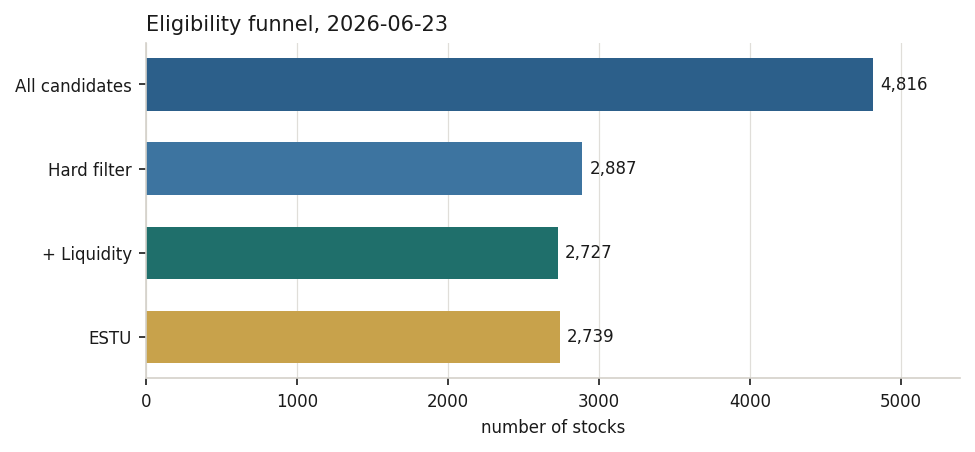
\includegraphics[width=\linewidth]{figures/estu_funnel.png}
\caption{The eligibility funnel for the latest signal date (personal build, 2026-06-23). The candidate universe narrows through the hard filters and the liquidity add gate; the ESTU sits marginally \emph{above} the strict add-gate count because the buffer's lenient retain rule keeps a few borderline members.}
\label{fig:funnel}
\end{figure}

\begin{remark}
The post-2010 in-ESTU small-segment share ($73.4\%$) sits far above MSCI's $\approx 14\%$ because ours is measured \emph{by count} within our cap-target proxy while MSCI's is \emph{by float capitalisation}. Both can be true at once; they answer different questions. The labels are informational; the cap target governs membership.
\end{remark}

\begin{exercise}
A junior quant filters the universe to ``isdelisted = false'' to ``keep it clean'' and reports a backtested factor Sharpe far above the team's. Name the bias, predict its sign on realised volatility forecasts, and give the one-line fix. \emph{(Hint: which firms are systematically missing from the pre-2010 cross-sections?)}
\end{exercise}

\begin{exercise}
A name IPO'd last week, so the ticker master (built before the IPO) has a \emph{null} category for it. The eligibility filter keeps only rows with category in the allowed set. What happens to this name, and why is it the opposite of the error you want? \emph{(Hint: a null fails an \texttt{is\_in} test silently.)}
\end{exercise}

\section{Liquidity: an ATVR proxy}\label{sec:liq}

\paragraph{Learning objectives.}
\begin{itemize}[nosep,leftmargin=1.4em]
  \item Define ATVR and the asymmetric $20\%$ add / $10\%$ retain thresholds.
  \item Construct a point-in-time trailing dollar-volume window using the right price field.
  \item Explain why a median (not a mean) and a minimum-populated window are used.
\end{itemize}

MSCI screens liquidity with the \textbf{Annual Traded Value Ratio (ATVR)}: annualised $\approx$3-month median daily dollar volume (ADTV) divided by float mcap, combined with a frequency-of-trading test. The thresholds are deliberately asymmetric --- \textbf{add} a name when $\text{ATVR}\ge 20\%$, but \textbf{retain} it until $\text{ATVR} < 10\%$ --- so that a name straddling the line is not thrown in and out every period.

Our proxy follows the same shape. Over a $\approx$3-month trailing window ($\approx 63$ trading days), compute daily dollar volume $d_{i,t}=\text{closeunadj}\times\text{volume}$ and take the \emph{median}, $\widetilde d_{i,t}$. The proxy ratio is
\[
\text{ATVR}_{i,t} = \frac{252\,\widetilde d_{i,t}}{m_{i,t}},
\]
where $252$ is the trading-day annualisation and the denominator is \emph{total} mcap $m_{i,t}$ --- our stand-in for MSCI's float mcap, inheriting the same float gap as everywhere else. The median (not the mean) is robust to earnings-day and catalyst spikes that would otherwise let one frantic session qualify an otherwise-thin name. We then apply the same $20\%/10\%$ add/retain asymmetry, and require a minimum-populated window (a majority of the window) --- which naturally keeps freshly-listed names out for roughly two months until they have enough history.

\begin{pitfall}
\textbf{Wrong price field.} Dollar volume must use \emph{unadjusted} close: $\text{closeunadj}\times\text{volume}$. Using \texttt{closeadj} (split- and dividend-adjusted) against raw volume mixes a back-adjusted price with present-day share counts --- nonsense dollars that diverge more the further back you look, biasing the liquidity screen across history.
\end{pitfall}

\begin{pitfall}
\textbf{Look-ahead.} The trailing window must use only days $\le t$ --- right-aligned, never centred. The clean implementation sorts the trading-day list once and bounds each window with \texttt{bisect\_right} at $\le t$, so no future session can ever leak into a signal-date liquidity figure. A centred or future-padded window is silent look-ahead that inflates in-sample fit and vanishes live.
\end{pitfall}

\begin{observed}
Post-2015, in-ESTU daily dollar volume has a median of $\approx\$18$M/day and a $10$th percentile of $\approx\$1.8$M/day (personal build, 2026-06-23) --- comfortably above any thin-trading regime, confirming the screen admits genuinely tradeable names.
\end{observed}

\begin{exercise}
A stock trades $\$1$M/day for $62$ days, then prints a single $\$60$M block on an acquisition rumour. Compare the mean and median dollar volume over the $63$-day window, and explain which one the liquidity screen should use and why. \emph{(Hint: a single observation moves the mean by $\approx \$60\text{M}/63$; what does it do to the median?)}
\end{exercise}

\section{Stability: an asymmetric buffer}\label{sec:stab}

\paragraph{Learning objectives.}
\begin{itemize}[nosep,leftmargin=1.4em]
  \item Explain hysteresis and why MSCI uses asymmetric size buffers ($\approx 1.8\times$ up, $1.0\times$ down).
  \item Describe our asymmetric rank-buffer proxy and the warm-start state it requires.
  \item Connect membership churn to bouncing standardisation moments and inflated style volatility.
\end{itemize}

MSCI engineers stability with \textbf{asymmetric size buffers}. To move \emph{up} a segment a name must clear a wider margin than it needs to fall \emph{out}: the published rule requires mcap above $\approx 1.8\times$ the cutoff to be promoted mid$\to$large, while only $< 1.0\times$ to be demoted large$\to$mid. The asymmetry is deliberate --- it is \emph{hysteresis}, a dead-band that prevents a name parked at the boundary from flipping segments on noise.

Our proxy is an \textbf{asymmetric rank buffer} with a few-hundred-rank hysteresis band. A name \emph{enters} only if its rank $r_{i,t}$ is inside the cap target and it is otherwise eligible; a \emph{current member} is \emph{retained} until its rank slips well past the band. Entry is strict, exit is lenient --- enter tight, exit loose, the same add/retain asymmetry we used for liquidity, now in rank space.

\begin{intuition}
Why bother with a buffer at all? Without one, roughly $5$--$10\%$ of the ESTU turns over every month purely from names oscillating across the boundary --- not because anything real changed. That churn is corrosive: bouncing membership $\to$ bouncing standardisation moments $\to$ bouncing exposures $\to$ spuriously inflated style-factor volatility, plus a jumpy Beta benchmark. The buffer roughly halves turnover to $1$--$2\%$, buying a quieter, more honest model for free.
\end{intuition}

\textbf{Two coupled buffers.} Stability is actually enforced by \emph{two} asymmetries acting together: the rank hysteresis band of this section \emph{and} the ATVR add/retain gap of Sec.\ \ref{sec:liq}. A prior member is dropped only when \emph{both} lenient conditions fail --- its rank slips past the band \emph{and} its ATVR falls below the retain floor. Equivalently, a borderline name is retained if \emph{either} buffer still holds it. The two independent dead-bands are what keep churn so low.

\textbf{State requirement.} The buffer is path-dependent: deciding whether to retain a name requires knowing whether it was a member \emph{last} month. The build therefore runs a chronological loop carrying last month's membership forward, and bootstraps the very first date with a strict cap target (no prior state exists yet). Unlike representation and liquidity --- which are functions of date $t$ alone and could be computed for every date in parallel --- the stability screen \emph{cannot} be parallelised across dates: each month consumes the previous month's output.

\begin{pitfall}
\textbf{Warm-start state.} Because membership depends on the previous month, restarting the build mid-history loses the carried-forward state and silently corrupts every retain decision afterward. Always rebuild from the calendar start --- it is cheap ($\approx 342$ monthly dates) and is the only way to reproduce the buffer exactly.
\end{pitfall}

\begin{observed}
Month-over-month one-way turnover averages $2.2\%$, with a $95$th percentile of $4.6\%$ and $98\%$ of months below the $5\%$ stability line (personal build, 2026-06-23; Figure~\ref{fig:churn}). The peak is $\approx 5.7\%$ at 2008-10, driven by crisis exits ($248$ names out). The resulting ESTU holds $\approx 2{,}500$ names (recent-era range $\approx 2{,}187$--$3{,}045$; earlier-era $\approx 1{,}791$--$2{,}760$), matching MSCI USA IMI breadth.
\end{observed}

\begin{figure}[htbp]
\centering
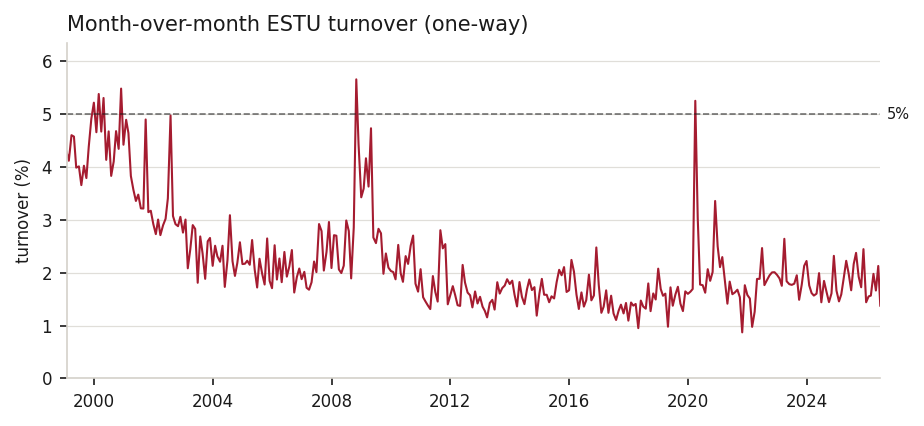
\includegraphics[width=\linewidth]{figures/estu_churn.png}
\caption{Month-over-month one-way ESTU turnover. The dashed line marks the $5\%$ stability threshold; turnover averages $\approx 2.2\%$ and stays below $5\%$ in $98\%$ of months. The $\approx 5.7\%$ peak (2008-10) is crisis-driven exits, not boundary noise.}
\label{fig:churn}
\end{figure}

\begin{remark}
The 2008-10 peak sits at the depth of the financial crisis, where genuine repricing and delistings (not boundary noise) pushed names out across the liquidity and cap screens --- a reminder that not all churn is bad churn.
\end{remark}

\begin{exercise}
With a symmetric rule, a name whose true rank is exactly at the cutoff and jitters by $\pm 1$ rank each month flips in and out every period. Show that widening the \emph{retain} threshold by a band $b$ while keeping the \emph{add} threshold fixed eliminates the flip for jitter $<b$, and explain the cost of choosing $b$ too large. \emph{(Hint: a member at rank cutoff${}+1$ is retained; when is it finally dropped, and what does a large $b$ do to who is left in?)}
\end{exercise}

\begin{exercise}
Widening the hysteresis band lowers churn. Name one benefit and one cost of widening it further, and explain why the band should be set a priori from first principles rather than tuned to maximise backtested factor performance. \emph{(Hint: what is being optimised, and on which sample, if you tune the band against factor returns?)}
\end{exercise}

\section{What the build run showed}\label{sec:run}

\paragraph{Learning objectives.}
\begin{itemize}[nosep,leftmargin=1.4em]
  \item Recite the validation battery and what each check guards against.
  \item State the deliverable scale of the artifact.
  \item Explain why the market-cap floor is reported qualitatively, not numerically.
\end{itemize}

The build ships with an eight-check validation battery, all green on the 2026-06-23 run:
\begin{enumerate}[nosep,leftmargin=1.6em]
  \item \textbf{ESTU size in band} --- the count stays within the expected range every date;
  \item \textbf{Month-over-month churn} --- turnover stays in the stable regime;
  \item \textbf{Mega-cap inclusion} --- AAPL, MSFT, GOOGL, JPM present every eligible month;
  \item \textbf{Mcap coverage} --- $99.3\%$ of the retain-eligible universe (vs.\ the $99\%$ target --- but measured on \emph{total}, not float, mcap);
  \item \textbf{Liquidity sanity} --- in-ESTU dollar volume well above thin-trading levels;
  \item \textbf{Segment proportions} --- the large/mid/small split is stable over time;
  \item \textbf{No PIT leaks} --- zero in-ESTU rows with null or zero mcap on the signal date;
  \item \textbf{Buffer invariants} --- the retained set is a subset of the prior membership; no name both enters and exits in the same month.
\end{enumerate}
Schema and disk read-back checks pass alongside these.

\begin{observed}
Validation: $8/8$ checks PASS; $0$ PIT leaks; schema and read-back PASS (personal build, 2026-06-23). Mega-caps appear in every eligible month (e.g.\ MSFT and JPM each $\approx 331$ months). Mcap coverage averages $99.3\%$ of the retain-eligible universe (post-2005 minimum $\approx 95.8\%$). Deliverable scale: $\approx 1.86$M panel rows, $\approx 825$k in-ESTU rows, $342$ monthly signal dates ($1998$-$01$-$30$ to $2026$-$06$-$23$), $\approx 17.4$k tickers.
\end{observed}

\begin{figure}[htbp]
\centering
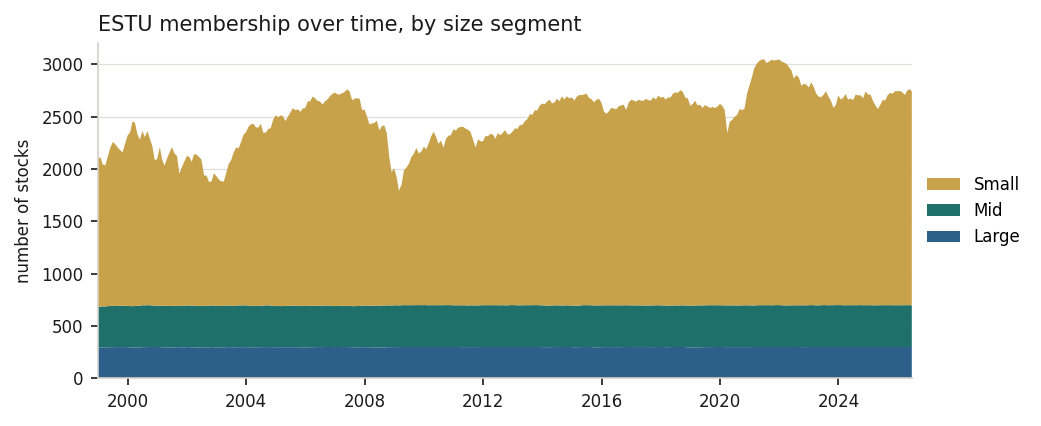
\includegraphics[width=\linewidth]{figures/estu_size.png}
\caption{ESTU membership over time, by size segment. Breadth holds near $\approx 2{,}500$ names --- the MSCI USA IMI scale --- dipping in the 2002 and 2008--09 drawdowns as names fail the liquidity and cap screens.}
\label{fig:size}
\end{figure}

\begin{remark}
Coverage admits two valid denominators. Against the \emph{retain-eligible} universe it is $99.3\%$; against the broader \emph{hard-filtered} universe it is $\approx 95.5\%$, with the $\approx 4.5\%$ gap being hard-filter passers whose ATVR sits below the retain floor --- illiquid names correctly screened out. The $99.3\%$ figure, read against the right denominator, is on-target rather than over-coverage.
\end{remark}

\begin{figure}[htbp]
\centering
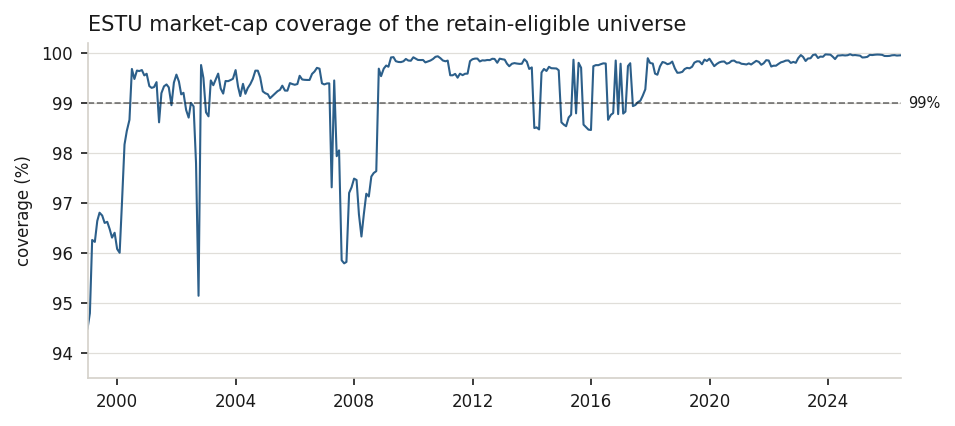
\includegraphics[width=\linewidth]{figures/estu_coverage.png}
\caption{ESTU market-cap coverage of the retain-eligible universe. The dashed line is the $99\%$ target; coverage holds at or above it for most of the sample (measured on total, not float, mcap).}
\label{fig:coverage}
\end{figure}

\begin{exercise}
Check~3 hard-codes four named mega-caps and asserts their presence every eligible month. Why is that a meaningful regression test, and what class of bug would it catch that the ESTU-size-in-band check (Check~1) would miss entirely? \emph{(Hint: a join or unit bug can keep the \emph{count} perfectly in band while dropping specific large names.)}
\end{exercise}

\textbf{The market-cap floor.} The effective floor --- a low-hundreds-of-millions effective market-cap floor --- binds on essentially every date: the cap-target proxy means the smallest included name sits near the floor by construction. What \emph{drifts} across the decades is the upper tail: the $5$th and $10$th percentiles of in-ESTU mcap climb steadily as the market grows. We report this qualitatively; the absolute floor is an invented proxy constant and is deliberately not printed.

\section{Summary, and one honest caveat}\label{sec:summary}

\paragraph{Learning objectives.}
\begin{itemize}[nosep,leftmargin=1.4em]
  \item Reconstruct ESTU membership as a right-to-left composition of the three screens.
  \item State the load-bearing limitation and the concrete lever that would fix it.
\end{itemize}

\begin{intuition}
Read membership right-to-left, as a composition:
\[
E = \underbrace{\text{stability buffer}}_{\text{over time}}\Big(\,\underbrace{\text{cap target}}_{\approx 99\%}\big(\,\underbrace{\text{liquidity screen}}_{\text{ATVR }20/10}\big(\,\underbrace{\text{hard-filtered, PIT-alive universe}}_{\text{PIT-alive, domestic, listed}}\,\big)\big)\Big).
\]
Start from every stock alive at $t$; keep domestic common stock (REITs included) on major exchanges; prune the thinly-traded with the ATVR proxy; take the cap target to hit $\approx 99\%$ coverage; then apply the buffer across time to damp churn. Each screen does one job, and the order matters --- liquidity before the cap target, the buffer last.
\end{intuition}

\begin{keyresult}
The single set $E_t$ feeds the standardisation moments, the Beta benchmark, the WLS sample, and every orthogonalisation sample. Build it once, set its parameters from first principles, and \emph{freeze} them --- every later set then inherits a consistent universe for free. The discipline is the deliverable.
\end{keyresult}

\begin{pitfall}
\textbf{The honest caveat.} The load-bearing limitation is \emph{total}-not-\emph{float} market cap. Total mcap inflates the effective size of founder- and insider-controlled names (a tightly-held firm looks larger and more includable than its tradeable float warrants), which biases both inclusion and cap weights, and feeds straight through to the ATVR denominator. The lever is procuring free-float data (MSCI or FactSet) and recomputing the cap target, the cap weights, and ATVR on float. Secondly, the proxy has never been validated against \emph{actual} IMI membership; the lever there is a licensed-constituent overlap study to measure where our screens and MSCI's disagree.
\end{pitfall}

\appendix
\section{Build pseudocode and decision table}\label{app:code}

The real build defines only report-printer helpers --- there are no named math kernels --- so the pseudocode below reads as \texttt{polars} expressions over a monthly signal-date loop, not invented function calls.

\medskip
\noindent\textbf{Monthly signal-date loop (point-in-time, state carried forward).}
{\footnotesize
\begin{verbatim}
import polars as pl
import numpy as np
from bisect import bisect_right

prev_estu = set()                      # warm-start state (empty on first date)
trading_days = sorted(all_days)        # sorted once for PIT window bounds

for t in monthly_signal_dates:         # chronological: state carried forward
    # --- alive + hard filters (PIT: a price row on t means alive) ---
    live = panel.filter(
        (pl.col("date") == t)
        & pl.col("category").is_in(ALLOWED_CATEGORIES)   # dom. common + REIT + 2nd class
        & pl.col("exchange").is_in(["NYSE", "NASDAQ", "NYSEMKT"])
    ).with_columns(
        (pl.col("marketcap") * 1_000_000).alias("mcap_usd")  # millions -> USD, once
    )

    # --- liquidity: PIT ~63-day trailing MEDIAN dollar volume -> ATVR proxy ---
    hi = bisect_right(trading_days, t)                  # days <= t only
    lo = hi - WINDOW                                    # window = ~63
    window_days = trading_days[max(lo, 0):hi]
    dv = (vol_panel
          .filter(pl.col("date").is_in(window_days))
          .with_columns((pl.col("closeunadj") * pl.col("volume")).alias("dollar_vol"))
          .group_by("ticker")
          .agg([pl.col("dollar_vol").median().alias("med_dv"),
                pl.col("dollar_vol").count().alias("n_obs")]))
    dv = dv.filter(pl.col("n_obs") >= MIN_OBS)          # majority-of-window populated

    # --- representation: rank by mcap; compute ATVR proxy ---
    ranked = (live.join(dv, on="ticker")
        .with_columns([
            ((252.0 * pl.col("med_dv")) / pl.col("mcap_usd")).alias("proxy_atvr"),
            pl.col("mcap_usd").rank(method="ordinal", descending=True).alias("mrank"),
        ]))

    # --- stability: TWO coupled asymmetries (rank band AND ATVR gap) ---
    enter  = ranked.filter((pl.col("mrank") <= TOPN)                # strict entry: rank
                           & (pl.col("proxy_atvr") >= ATVR_ADD))    # strict entry: ATVR
    retain = ranked.filter((pl.col("mrank") <= TOPN + BUFFER)       # lenient retain: rank
                           & (pl.col("proxy_atvr") >= ATVR_RETAIN)  # lenient retain: ATVR
                           & pl.col("ticker").is_in(list(prev_estu)))
    estu_t = set(enter["ticker"]) | set(retain["ticker"])

    write_estu(t, estu_t)
    prev_estu = estu_t                                  # carry state to next month
\end{verbatim}
}

\smallskip
\noindent The judgment calls that are \emph{not} dictated by USE4/MSCI --- the proxy thresholds we set from first principles and then froze --- are catalogued below. Proxy constants are abstracted; only published or measured quantities appear numerically.

\begin{center}
\small
\begin{tabular}{@{}p{0.27\linewidth}p{0.40\linewidth}p{0.27\linewidth}@{}}
\toprule
Decision & Choice & Rationale \\
\midrule
mcap input & total mcap (no float available) & Sharadar gap; see caveat (Sec.\ \ref{sec:summary}) \\
Alive test & price row on $t$ & avoids survivorship; never use \texttt{isdelisted} \\
Security categories & domestic common stock + REITs + secondary class & matches MSCI IMI; REITs load-bearing for yield/leverage \\
Share classes & kept separate (own permaticker) & GOOG/GOOGL, BRK.A/BRK.B not consolidated \\
Cap target & fixed top-$N$ (a few thousand) & stable, debuggable proxy for the $99\%$ cumulative cutoff \\
Liquidity window & $\approx 63$ trading days, days $\le t$ & MSCI 3-month ADTV; PIT, right-aligned \\
Liquidity statistic & median dollar volume & robust to catalyst/earnings spikes \\
Add / retain & ATVR $\ge 20\%$ add, $< 10\%$ retain & MSCI published asymmetry \\
Min.\ window obs & majority-of-window populated & keeps freshly-listed names out $\approx 2$ months \\
Stability buffer & asymmetric rank band (few-hundred ranks) + ATVR gap & two coupled hysteresis bands; mirrors MSCI $1.8\times/1.0\times$ \\
Rebalance & monthly; carry membership forward & damps churn; needs warm-start state \\
Calendar start & 1998 & data-driven history start \\
\bottomrule
\end{tabular}
\end{center}

\begin{center}\small\itshape
References: Menchero, J., Orr, D.J., \& Wang, J. (2011), \emph{The Barra US Equity Model (USE4)} --- Methodology Notes (Sec.\ 3.1, 2.3) and Empirical Notes (Sec.\ 3.1). MSCI Global Investable Market Indexes (GIMI) Methodology (public principles: representation, liquidity, stability). Build figures from personal build run dated 2026-06-23.
\end{center}

\end{document}
